\documentclass{scrarticle}

\usepackage{amsmath}
\usepackage{graphicx}
\usepackage{microtype}
\usepackage{hyperref}

\begin{document}
\section{Question about interesting observation}

When computing the function, we sum over matrix elements
\begin{equation}
  \label{eq:1}
  \chi^{xy} \propto \sum\limits_{mn}^{} J^x_{mn} T_{mn}^{y0},
\end{equation}
where \( m,n \) are Landau levels.
I denote a term of the sum a ``transition'', as is usual.
Usually in conductivity computations, one gets the \emph{Diatomic} selection rule \( |m| = |n| \pm 1 \), i.e. we only have transitions between Landau levels whose number differ by one.
For untilted cones, we get this selection rule.
At \( T\to 0 \), the only energetically allowed transitions are further restricted to those of opposite sign.
However, for tilted cones, we do not get the Diatomic selection rule, and thus we have to consider in the sum transitions between all levels, see figure \ref{fig:contribs}.

\begin{figure}[p]
  \centering
  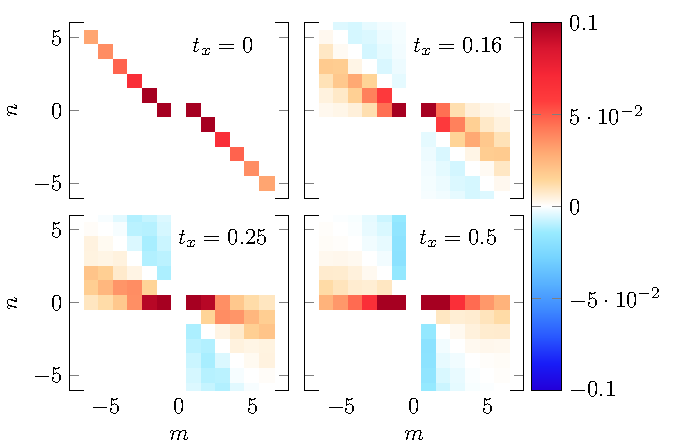
\includegraphics[width=\textwidth]{../Thesis/figures/external/contribmn-P}
  \caption{Contributions to \( \gamma_N \) from \( m\to n \) transitions for different values of \( t_x \).
    In order to retain contrast, the color values are capped at \( 0.1 \), meaning that the \( \gamma_0 \) contributions are clipped.
    \label{fig:contribs}
    }
\end{figure}

\begin{figure}[p]
  \centering
  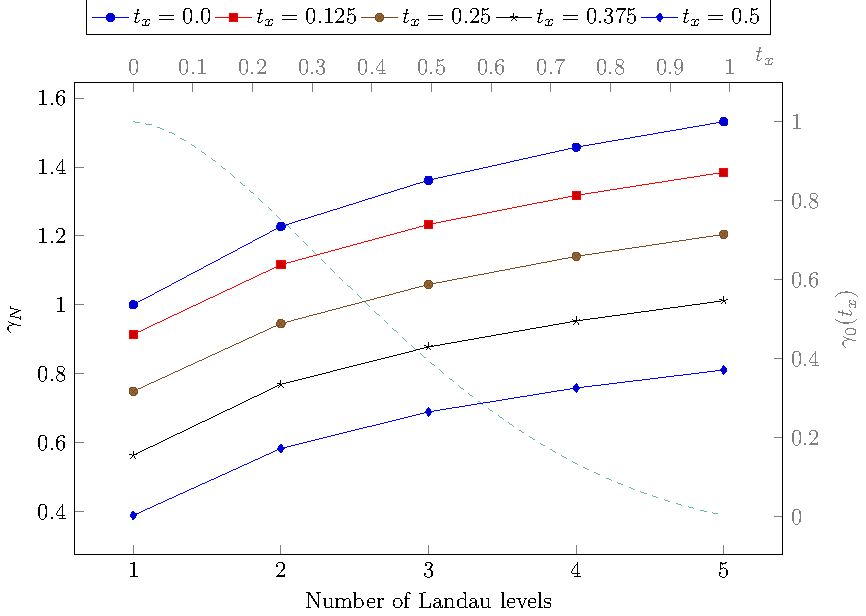
\includegraphics[width=\textwidth]{../Thesis/figures/external/contribtx}
  \caption{\label{fig:contribN}}
\end{figure}

In the thesis, I defined the numerical prefactor to the response \( \gamma_N \) which is the sum of all interactions up to LL \( N \), see upper left pane in figure \ref{fig:contribs}.
This gives the prefactor shown in figure \ref{fig:contribN};
the prefactor is reduced as the tilt is increased.
\emph{However}, I got the idea to consier only \( 0\to n \) transitions, as opposed to any \( m\to n \).
The reason why this might make sense, is that for large magnetic field only the zeroth LL is filled.
Doing this, we get the result shown in figure \ref{fig:zerothll}.
Now this is very interesting!!

However, I am uncertain if this procedure makes sense.
I will think a bit more about it, but hope that you also can think of this.
The reason I am uncertain, is that we almost always have the diatomic selection rule, so exactly how to make the LL cutoff without it I am uncertain about.

\begin{figure}[p]
  \centering
  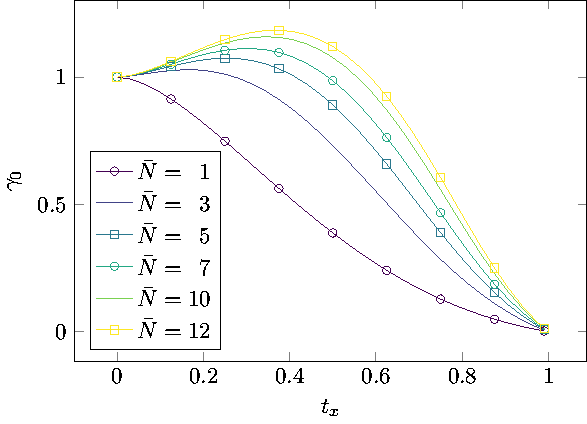
\includegraphics[width=\textwidth]{../Thesis/figures/external/contribtx-zerothll}
  f
  \caption{Numerically computed values of the prefactor \( \gamma_N \) with only the \( 0 \to i \) up to \( N \) transitions included for perpendicular tilt \( t_x \).
    The contribution is even in \( t_x \), and vanish as \( |t_x| \to 1 \).
    \label{fig:zerothll}
  }
\end{figure}
\end{document}
